%\chapter{Desenvolvimento do Trabalho} \label{cap:desenvolvimento}

%\section{Tecnologias Utilizadas}
%Durante o desenvolvimento do trabalho, são utilizadas tecnologias e ferramentas adequadas. Essa seção deve apresentar as tecnologias e ferramentas mais relevantes, utilizadas no desenvolvimento. 

%\section{Projeto e Implementação}
%Descrever os resultados do projeto e da implementação do trabalho, com justificativas das decisões tomadas.

%\section{Testes e Avaliação}
%Descrever o procedimento da avaliação do trabalho (teste de hardware, teste de software, teste de módulo, teste de integração, teste de validação), de acordo com o tipo do sistema, com o apoio do orientador, se necessário.

\chapter{Desenvolvimento} \label{cap:desenvolvimento}
 % ===================================================================
\section{Cronograma}
% ===================================================================
 
O projeto é executado de abril a setembro de 2026, dividido em duas entregas
mensais. A \autoref{tab:cronograma-cap-desenvolvimento} e a \autoref{fig:diagrama-gantt-cap-desenvolvimento} apresentam o cronograma detalhado.
 
\begin{longtable}{p{1.8cm} p{6cm} p{6cm}}
\caption{Cronograma das atividades planejadas} \label{tab:cronograma-cap-desenvolvimento} \\
\toprule
\textbf{Mês} & \textbf{Entrega 1} & \textbf{Entrega 2} \\
\midrule
\endfirsthead

\toprule
\textbf{Mês} & \textbf{Entrega 1} & \textbf{Entrega 2} \\
\midrule
\endhead
 
\textbf{Abril} &
\textit{Setup} do projeto com FreeRTOS / ESP-IDF; implementação do \texttt{MockDataCollector}; estudos sobre a plataforma. &
Início da escrita do TCC: Introdução, Fundamentação Teórica (OBD-II, CAN, segurança) e Modelagem de Ameaças. \\ \hline
 
\textbf{Maio} &
Comunicação OBD-II via CAN (ESP32 + transceptor CAN conectado a simulador OBD-II); leitura de PIDs reais. &
Comunicação ESP32 $\leftrightarrow$ App, recebimento de dados em tempo real (via Wi-Fi ou BLE). \\ \hline
 
\textbf{Junho} &
Testes de segurança iniciais (\textit{Donglescope}); implementação do protocolo de autenticação mútua entre App e \textit{dongle}. &
Cifração do tráfego entre App e \textit{dongle} (AES-GCM + ECDH); integração com módulo de autenticação. \\ \hline
 
\textbf{Julho} &
Testes de segurança completos; redação dos capítulos de Arquitetura e Análise Comparativa com \textit{dongles} comerciais. &
Desenvolvimento das telas principais do App (visualização de PIDs, DTCs, odômetro). \\ \hline
 
\textbf{Agosto} &
\textit{Buffer} para absorção de atrasos e ajustes. &
\textit{Buffer} para absorção de atrasos e ajustes. \\ \hline
 
\textbf{Setembro} &
Consolidação da versão final do TCC; revisão geral do texto, correções e formatação. &
--- \\
 
\bottomrule
\end{longtable}

\begin{figure}[H]
    \centering
    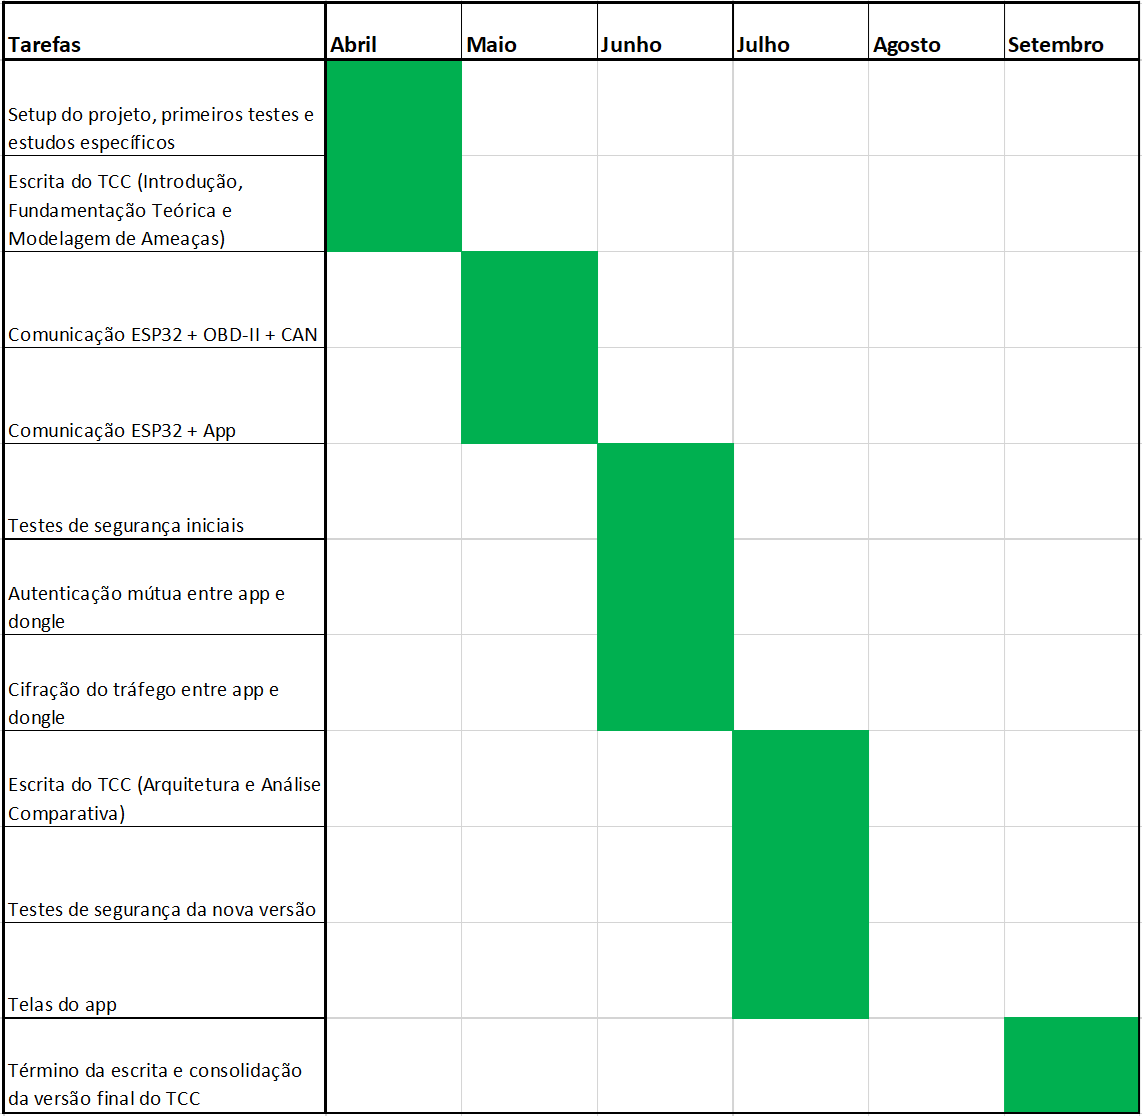
\includegraphics[width=0.9\linewidth]{assets/cap5-desenvolvimento/gantt.png}
    \caption{Diagrama de Gantt das atividades planejadas}
    \label{fig:diagrama-gantt-cap-desenvolvimento}
\end{figure}
